\documentclass{beamer}

\usepackage[utf8]{inputenc}
\renewcommand{\familydefault}{\sfdefault}
\usepackage{default}
\usepackage{animate}
\usepackage{graphicx}
\graphicspath{{../../../Img/}}
\usepackage{color}
\usepackage{textpos}
\definecolor{light-gray}{gray}{0.95}

\logo{
\includegraphics[height=0.8cm]{GlasgowLogo.png}\vspace{220pt}}

\usetheme{CambridgeUS}
\usecolortheme{lily}

\setbeamercolor{footline}{bg=gray}

\setbeamertemplate{frametitle}
{
\begin{flushleft}
\color{black}
\textbf{\normalsize\insertframetitle}
\end{flushleft}
}

\setbeamertemplate{titlepage}
{
\begin{flushleft}
\color{black}
\textbf{\normalsize\insertframetitle}
\end{flushleft}
}

\defbeamertemplate*{title page}{customized}
{
  \centering{
  \fontsize{15pt}{12pt}\textbf\inserttitle\par
  \insertsubtitle\par
  \bigskip
  \insertauthor\par
  \insertdate\par
  }
}

\setbeamertemplate{footline}
{
  \leavevmode%
  \hbox{%
  \begin{beamercolorbox}[wd=.4\paperwidth,ht=2.25ex,dp=1ex,center]{author in head/foot}%
    \usebeamerfont{author in head/foot}\insertshortauthor
  \end{beamercolorbox}%
  \begin{beamercolorbox}[wd=.6\paperwidth,ht=2.25ex,dp=1ex,center]{footline}%
    \usebeamerfont{title in head/foot}{\insertframenumber{} / \inserttotalframenumber}
  \end{beamercolorbox}}%
  \vskip0pt%
}

\setbeamertemplate{headline}
{
  \leavevmode%
  \hbox{%
  \begin{beamercolorbox}[wd=.4\paperwidth,ht=2.25ex,dp=1ex,center]{author in head/foot}%
    \usebeamerfont{author in head/foot}\insertsection
  \end{beamercolorbox}%
  \begin{beamercolorbox}[wd=.6\paperwidth,ht=2.25ex,dp=1ex,center]{footline}%
    \usebeamerfont{title in head/foot}Electrostatics Project\hspace*{3em}
  \end{beamercolorbox}}%
  \vskip0pt%
}


\setbeamertemplate{navigation symbols}{}

\title{Numerical solutions to electrostatic problems: Efficient Algorithm Design, Project Structure, and Auxilliary Classes}
\author{David Muir}
\institute{University of Glasgow}
\date{March 14th, 2013}

\begin{document}

{
\setbeamertemplate{headline}{}
\setbeamertemplate{footline}{}
\begin{frame}
  \titlepage
\end{frame}
\addtocounter{framenumber}{-1}

}

\section{Introduction}

\begin{frame}{Introduction}
    \begin{itemize}
        \item Optimising an existing implementation of the Finite Difference algorithm. 
        \item Defining the project structure and ensuring proper separation of concerns
        \item Creating auxilliary classes
            \begin{itemize}
                \item To read pixel data from bitmap image files
                \item To output grid information to the gnuplot graphing program
            \end{itemize}
    \end{itemize}
\end{frame}

\section{Algorithm Optimisation}

\begin{frame}{Fast Finite Difference}
    The Fast Finite Difference algorithm was an attempt to optimise the existing Finite Difference algorithm by Karl Nordstrom.

    The requirements for this algorithm were as follows,
    \begin{itemize}
        \item To reduce the runtime of the Finite Difference algorithm by an appreciable degree so as to allow more time-effective computations.
        \item To arrive at exactly the same approximation as the previous algorithm.
    \end{itemize}
\end{frame}

\begin{frame}{Performance}
    \begin{figure}
        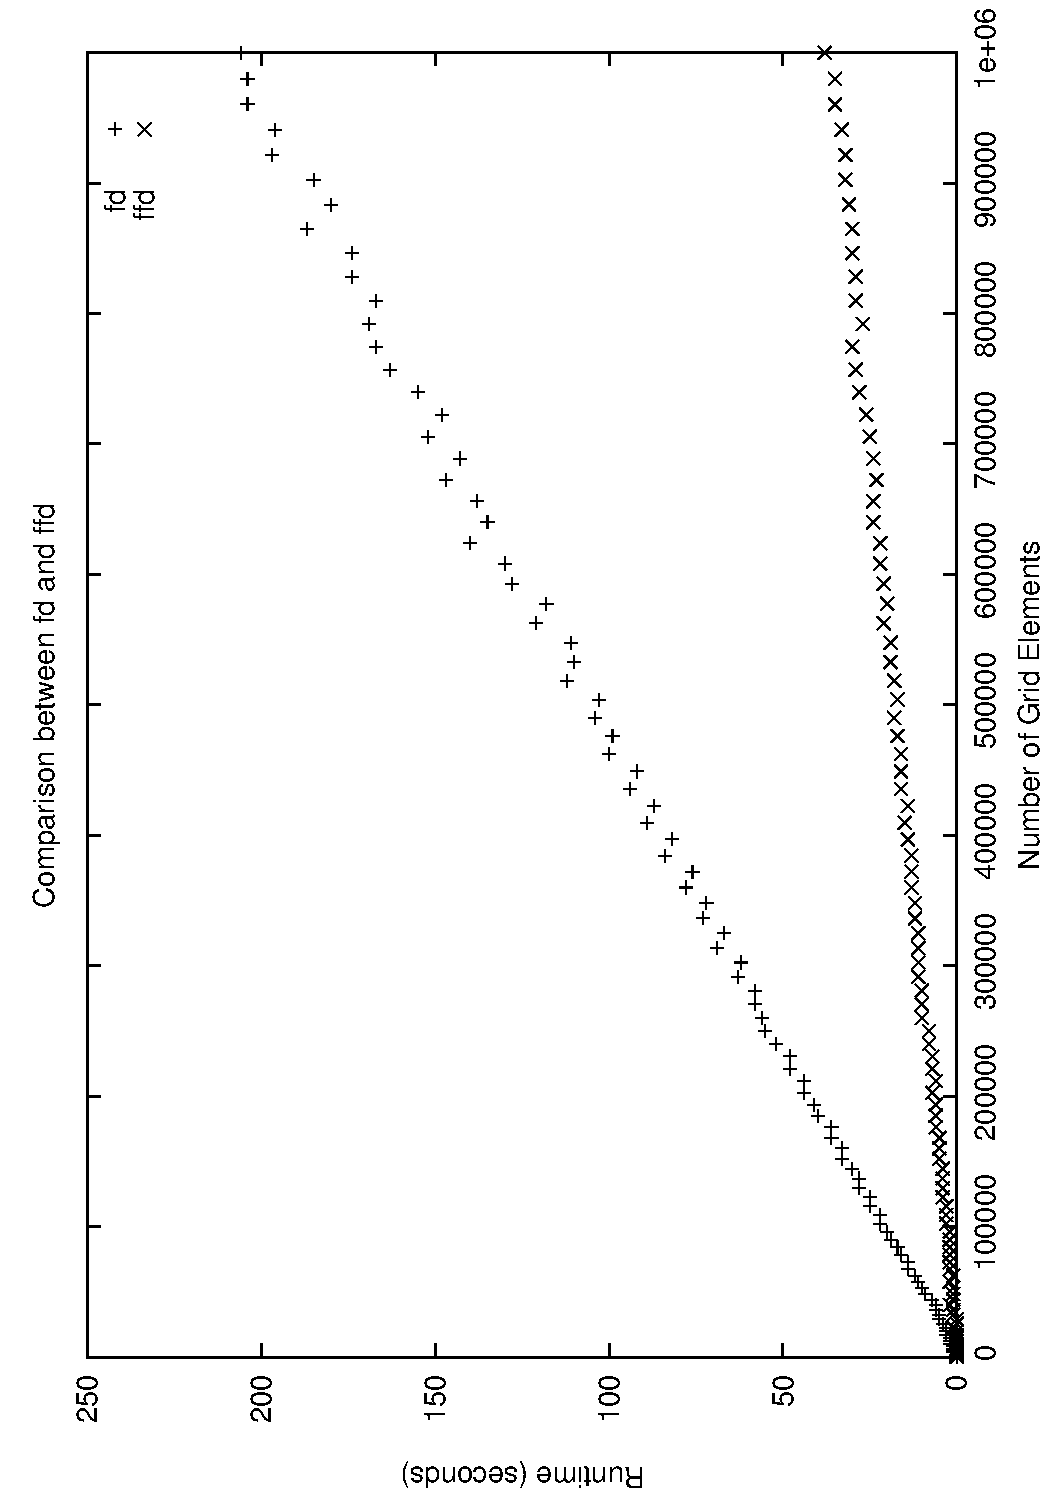
\includegraphics[angle=-90,width=0.7\textwidth]{fd_ffd_comparison.pdf}
    \end{figure}
    \em{Run on an i5-3317U@1.7GHz for 10,000 iterations per grid size and Ofast compiler optimsations on both algorithms.}
\end{frame}

\begin{frame}{Performance Optimisations}
    To attain the performance increases desired these traits were selected.
    \begin{itemize}
        \item Reduce repeated calculations
        \item Reduce memory access
        \item Reduce object creation
        \item Pass by reference rather than value
    \end{itemize}
\end{frame}

\begin{frame}{Non-diminishing Accuracy}
    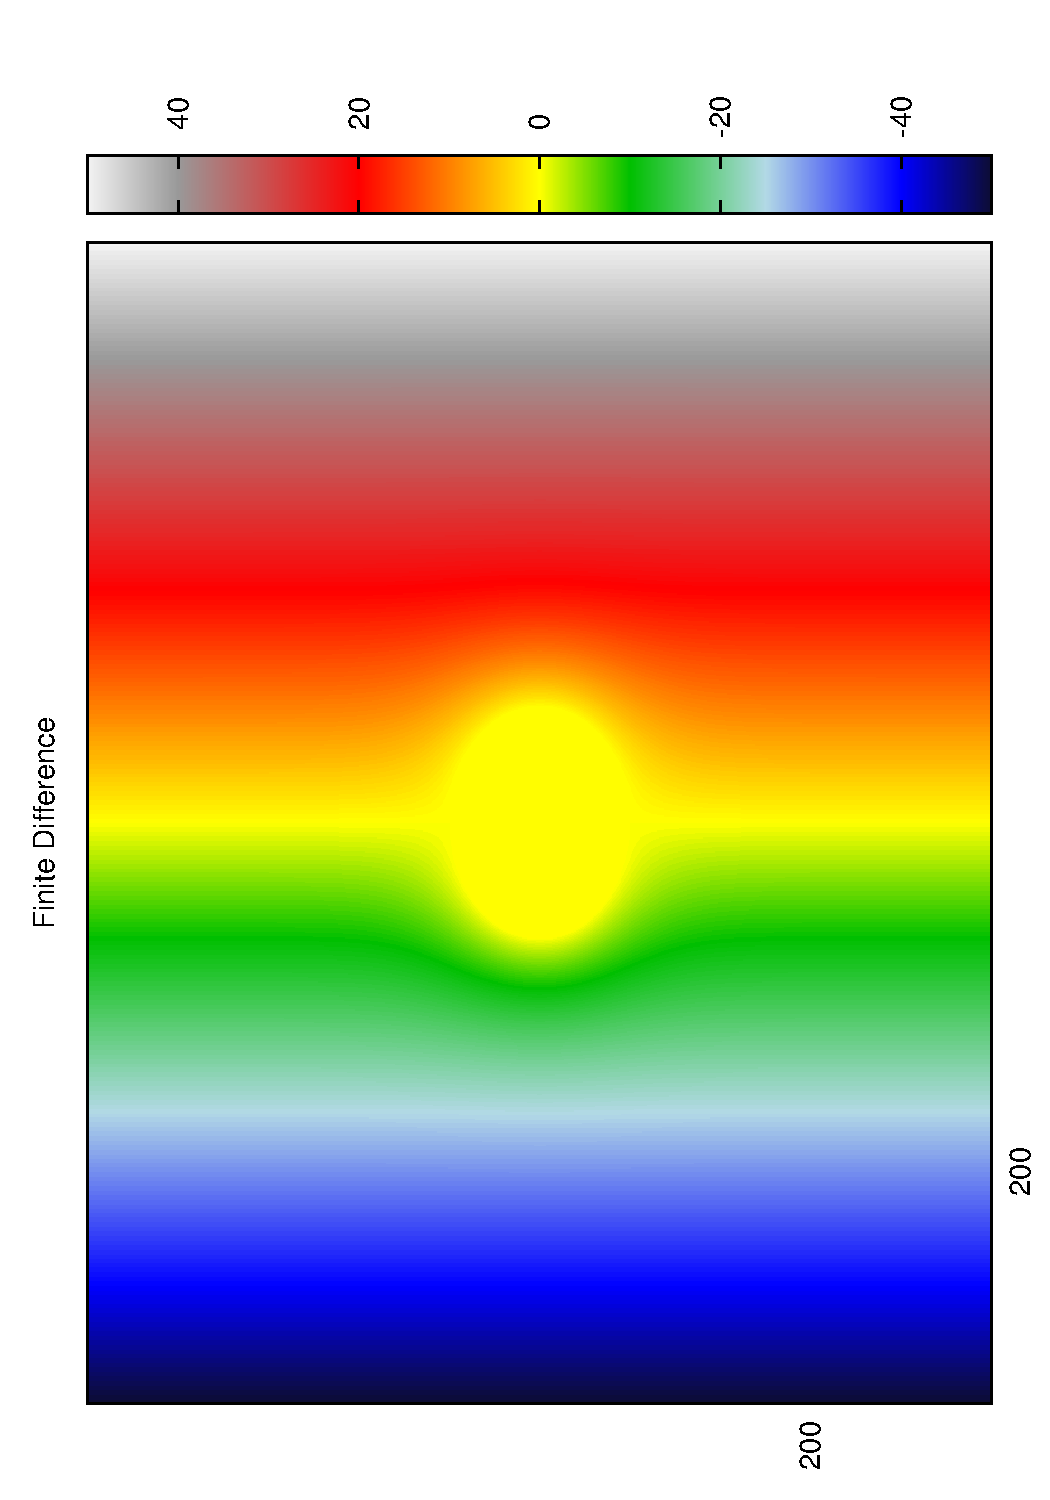
\includegraphics[angle=-90,width=0.5\textwidth]{fd.pdf}
    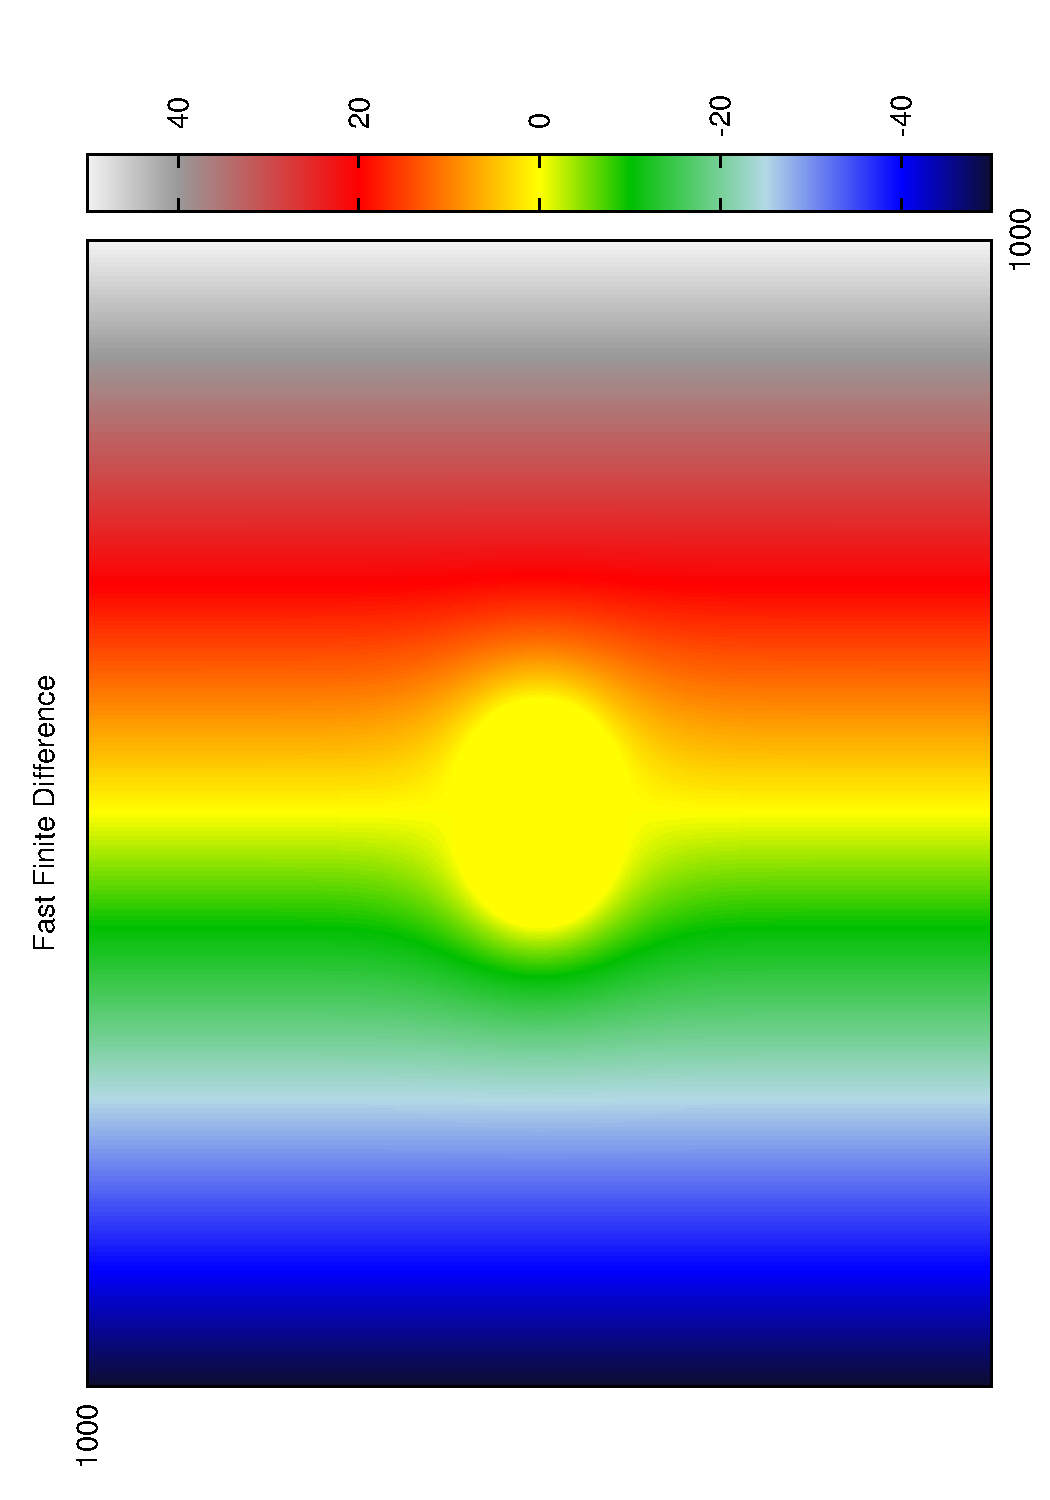
\includegraphics[angle=-90,width=0.5\textwidth]{ffd.pdf}
\end{frame} 

\section{Project Structure}

\begin{frame}{Project Structure}
    For a medium size project such as this a well defined structure is an important concern.
    Without the proper seperation of concerns the project would soon become an unmaintainable mess.
\end{frame}

\begin{frame}
   The code is split up into the following directories:
   \begin{itemize}
        \item Algorithms
        \item Errors
        \item Structures
        \item Utils
    \end{itemize}
\end{frame}

\section{Auxilliary Classes}

\begin{frame}{Gnuplot}
    \begin{itemize}
        \item The Gnuplot class was created to facilate in-app usage of the Gnuplot program. With an aim to allow more automation and reduce our dependancy on additional scripting.
        \item The class opens a connection to Gnuplot and allows passing of commands, comments, and Grid data directly to the program.
        \item There is also the option to read commands from a script and save to a script
    \end{itemize}
\end{frame}

\begin{frame}{Bmp Reader}
    \begin{itemize}
        \item The Bmp Reader class was created to allow us to input user defined shapes as a standard format
        \item The class reads in the pixel data of the bitmap and takes darker sections as referring to boundaries.
        \item The class will then create and return a grid populated by the bitmap
    \end{itemize}
\end{frame}

\begin{frame}
    \begin{figure}
        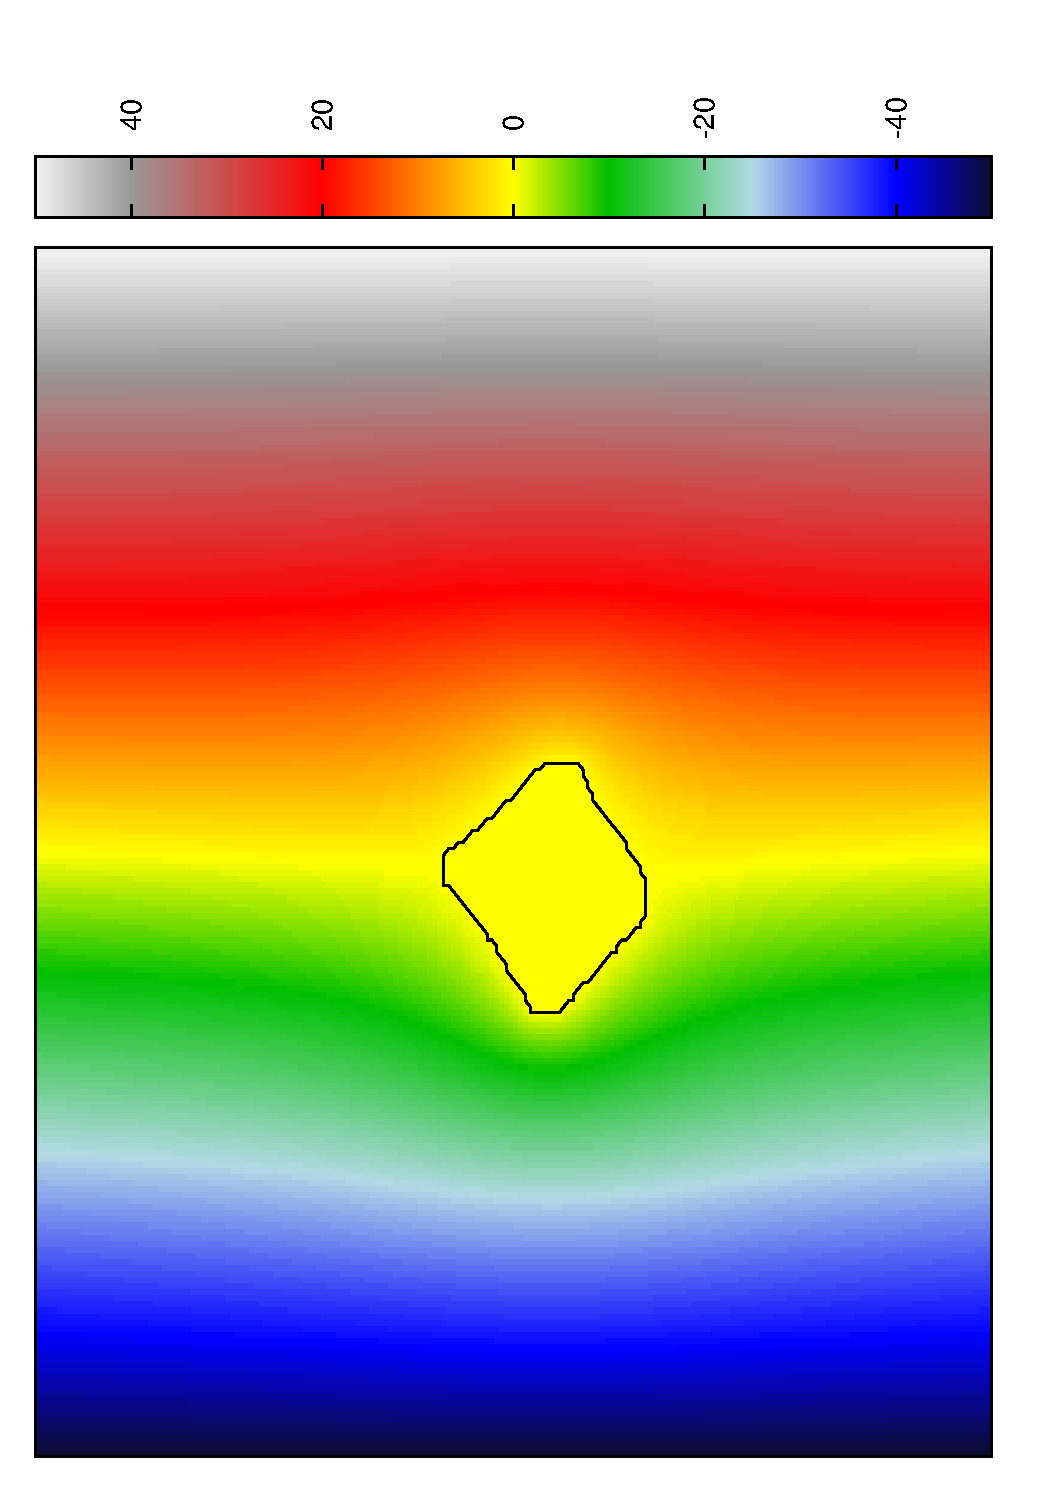
\includegraphics[angle=-90,width=\textwidth]{bmp.pdf}
    \end{figure}
\end{frame}

\end{document}
